% Preamble
% ---
\documentclass[paper=a4, fontsize=11pt]{scrartcl}

% Packages
% ---
\usepackage{geometry}
\geometry{
  a4paper,
  left=15mm,
  right=15mm,
  headheight=50mm,
  top=30mm,
  bottom=16mm,
  footskip=10mm
}
\usepackage{graphicx}
\usepackage[utf8]{inputenc}     % UTF-8 support
\usepackage{amsmath,amsfonts}   % Advanced math typesetting
\usepackage{gauss}              % Matrices reduction operations
\usepackage{lastpage}           % Reference to last page
\usepackage[parfill]{parskip}   % No indent at start of new line
\usepackage{hyperref}           % Table of contents with clickable links
\usepackage{subfig}             % Figure repartition on page
\usepackage{ragged2e}
\usepackage[T1]{fontenc}
\usepackage[french]{babel}
\usepackage{listings}           % Source code formatting and highlighting
\usepackage{float}              % Positioning of figures
\usepackage{xcolor}             % Color in code blocks

\newcommand{\ts}{\textsuperscript} % shortcut

% Code Block style
\definecolor{codegreen}{rgb}{0,0.6,0}
\definecolor{codegray}{rgb}{0.5,0.5,0.5}
\definecolor{codepurple}{rgb}{0.58,0,0.82}
\definecolor{backcolour}{rgb}{0.95,0.95,0.92}
\lstdefinestyle{mystyle}{
    backgroundcolor=\color{backcolour},   
    commentstyle=\color{codegreen},
    keywordstyle=\color{magenta},
    numberstyle=\tiny\color{codegray},
    stringstyle=\color{codepurple},
    basicstyle=\ttfamily\footnotesize,
    breakatwhitespace=false,         
    breaklines=true,                 
    captionpos=b,                    
    keepspaces=true,                 
    numbers=left,                    
    numbersep=5pt,                  
    showspaces=false,                
    showstringspaces=false,
    showtabs=false,                  
    tabsize=2
}
\lstset{style=mystyle}

\frenchbsetup{StandardLists=true}
\hypersetup{
    colorlinks,
    citecolor=black,
    filecolor=black,
    linkcolor=black,
    urlcolor=black
}
\usepackage{fancyhdr}           % Create headers and footers
\pagestyle{fancy}

% Header and footer things
% ---
% Header of all pages
\lhead{
\includegraphics[width=5cm]{img/logo.png}}
\rhead{Jael Dubey}

% Footer of all pages
\renewcommand{\footrulewidth}{0.4pt}
\lfoot{Système de logging multi-niveau}
\cfoot{}
\rfoot{Page \textbf{\thepage} \ sur \textbf{\pageref{LastPage}}}

% Header and footer of the first page
\fancypagestyle{firstpage}{
  \renewcommand{\headrulewidth}{0pt}
  \lhead{
\includegraphics[width=5cm]{img/logo.png}}
  \rhead{Département : Technologies de l'information et de la communication\linebreak Filière : Informatique et systèmes de communication\linebreak Orientation : Informatique logicielle}
  \renewcommand{\footrulewidth}{0pt}
  \lfoot{}
  \rfoot{}
}


% Modify the \paragraph behavior
\makeatletter
\renewcommand\paragraph{\@startsection{paragraph}{4}{\z@}%
            {-2.5ex\@plus -1ex \@minus -.25ex}%
            {1.25ex \@plus .25ex}%
            {\normalfont\normalsize\bfseries}}
\makeatother
\setcounter{secnumdepth}{4} % how many sectioning levels to assign numbers to
\setcounter{tocdepth}{4}    % how many sectioning levels to show in ToC


% Document
% ---
\begin{document}

% Don't number sections
% \setcounter{secnumdepth}{0}

% Title page ========================================================
\begin{titlepage}
  \thispagestyle{firstpage}
  \begin{center}
    \vspace*{5cm}
    
    \Huge
    \textbf{Travail de Bachelor}

    \vspace{1.5cm}
    \LARGE
    Analyse et implémentation d'un système de logging multi-niveau pour une plateforme Smart Grid
  \end{center}

  \vspace{6cm}
  \begin{tabbing}
    \linespread{3}\textbf{Étudiant :} \hspace{12em} \= Jael Dubey\\\\

    \textbf{Travail proposé par :} \> Jonathan Bischof\\
    \> DEPsys SA\\
    \> Route du Verney 20B\\
    \> 1070 Puidoux\\\\

    \textbf{Enseignant responsable :} \> Nastaran Fatemi\\\\

    \textbf{Année académique :} \> 2019-2020
  \end{tabbing}

  \vspace{3cm}
  \begin{flushright}
    Yverdon-les-Bains, le \textit{JOUR} \textit{MOIS} 2020
  \end{flushright}
\end{titlepage}

\newpage

% Cahier des charges ================================================
\section{Cahier des charges}
\subsection{Résumé du problème}
DEPsys est une entreprise Suisse leader technologique du marché énergétique. Fondée en 2012 et basée à Puidoux, elle fournit des solutions évolutives basées sur sa plateforme GridEye permettant aux réseaux de distribution d'énergie traditionnels de faire face aux nouvelles contraintes de la production décentralisée des sources d'énergie renouvelable, tels que les systèmes photovoltaïques et les technologies de mobilité électrique.

La plateforme GridEye offre une solution technologique innovatrice pour les gestionnaires de réseau de distribution (GRD, p. ex. Romande Énergie). Positionné de manière unique avec sa simplicité de déploiement, c'est la seule solution réellement Plug \& Play qui évite tous les problèmes d'installation. La surveillance du réseau électrique en temps réel et les statistiques fournissent des informations détaillées sur les conditions du réseau. Les algorithmes de contrôle et de gestion garantissent la qualité et la stabilité du réseau.

Ce Travail de Bachelor consiste en une évaluation de différentes technologies de logging et de l'analyse des performances, pour ensuite mettre en place la meilleure solution pour l'infrastructure GridEye.

\subsection{Étapes de réalisation du projet}

\begin{itemize}
    \item Étude des systèmes de gestion de logs actuels.
    \subitem Choix des systèmes à évaluer.
    \item Évaluation théorique des systèmes.
    \item Prise en main et configuration des outils pour une comparaison théorique \& pratique.
    \subitem Choix d'un système.
    \item Implémentation d'un cas d'utilisation concret fourni par DEPsys.
    \subitem Avec un programme de simulation minimaliste de la plateforme GridEye.
    \item Implémentation d'une démonstration de faisabilité (Proof of Concept, PoC).
    \item Implémentation de librairies (SDK) pour l'interfaçage avec le Back-End de la solution GridEye (puis Front-End, puis outils externes).
\end{itemize}

\subsection{Informations diverses et technologies}
Les logs sont constitués de plusieurs types (System, User Action, Notification, ...) avec différents niveaux de priorités (debug, info, ...). Les logs utilisateurs doivent pouvoir être consultés depuis le Front-End, alors que les logs systèmes peuvent être accessible depuis une dashboard interne. Les notifications, dépendant du niveau de priorité, doivent pouvoir être transmises en temps réel aux gestionnaire de réseau de distribution électrique  par e-mail, notification push, etc. ou sous forme de rapport journalier/hebdomadaire. La mise en place de librairies (SDK) est nécessaire pour communiquer avec les différents composants de l'infrastructure. Le but étant de pouvoir s'interfacer avec l'infrastructure actuelle afin de pouvoir remplacer la solution de logging actuelle.

Technologies:

\begin{itemize}
    \item Base de données : SQL, JSON, ... (dépendant de la solution choisie).
    \item Back-End : Java
    \item Front-End : Javascript 
    \item Outils externes : Python 3
\end{itemize}
\newpage

% Contents page =====================================================
\renewcommand{\contentsname}{Table des matières}
\tableofcontents

\newpage
% Document start ====================================================

\section{Introduction}
\section{Évaluation}

\subsection{Critères d'évaluation}

Pour réaliser une évaluation de différents système de gestion de log, il faut obligatoirement choisir des critères d'évaluation. Ces critères se basent sur deux sources. La première étant les demandes formulées par DEPsys, et la deuxième provient des différentes fonctionnalités nécessaires à un système de gestion de logs. Voici les critères retenus :

\begin{itemize}\itemsep0pt \parskip0pt \parsep0pt
\item La collecte des logs
\subitem Approche minimaliste ou maximaliste, est-ce que le système installe un agent sur le dispositif émetteur de log qui lui envoie uniquement les informations les plus importantes (approche minimaliste, méthode PUSH), ou est-ce que le système reçoit tous les logs et les enregistre tous (approche maximaliste, méthode PULL) ?\\
\item L'agrégation centralisée des logs
\subitem L'agrégation des logs est un défi, car après avoir collecté les logs, il faut tous les regrouper dans un même endroit, alors qu'ils peuvent avoir des formats différents. De plus, ils peuvent être généré très rapidement (s'exprime en EPS, Event Per Second), il faut donc être capable de traiter et regrouper ces logs de manière efficace.\\
\item Le stockage à long terme et la durée de rétention des logs
\subitem Après avoir agrégé ces informations, il faut maintenant faire des choix quant à leur stockage. L'idéal serait de garder tous les logs indéfiniment, mais chaque information stockée à un coût. Il faut donc avoir une stratégie de rétention qui permette de supprimer ou garder tel type de log.\\
\item La rotation des fichiers de logs
\subitem La rotation consiste à rendre automatique la stratégie de rétention et/ou de stockage des logs.\\
\item L'analyse des logs (en temps réel et en vrac après une période de stockage)
\subitem L'analyse des logs est, en quelque sorte, le but de tout le système de gestion de logs. En effet, il ne sert à rien de stocker de l'information sur un système si l'on en fait rien. L'analyse est donc la pour synthétiser les informations contenues dans les logs.\\
\item Les rapports
\subitem Il doit être possible pour un système de gestion des logs d'effectuer des recherches sur les informations stockées et de rédiger des rapports.\\
\item Visionnage et gestion des alertes
\subitem Un des buts d'un système de gestion de logs est de pouvoir réagir très vite à un problème, voire même de l'anticiper. Ceci passe par une émission d'alerte et d'une possibilité de visionnage des données, si possible en temps réel.\\
\item Popularité
\subitem Voici un critère qui change en permanence, mais qui a son importance lors d'un choix d'outil informatique. En effet, un logiciel sur le déclin sera de plus en plus dur à supporter, alors qu'un outil trop jeune n'a souvent que trop peu d'utilisateurs qui pourraient partager leurs connaissances sur les forums. L'idéal étant donc un logiciel populaire et qui est en pleine croissance.
\end{itemize}

En plus de ces critères, les coûts d'utilisation seront évalués.\\

\subsection{Choix des différents systèmes à évaluer}

Comme pour le choix des critères d'évaluation, les différents systèmes qui vont être analysés ont été définis soit par DEPsys, soit par des recherches dans les nombreux classement de \og Log Management Tools \fg disponible sur internet.\\
Quatre classements différents ont été sélectionnés afin d'avoir plusieurs avis différents, tout en restant dans une quantité raisonnable d'analyses. Les classements qui allaient être utilisés devaient être neutre. On entend par là que le site réalisant le classement ne doit pas proposer, par exemple, une solution cloud utilisant un certain outil de gestion de log, auquel cas son classement serait forcément biaisé. Il fallait également que le classement soi récent, étant donné la vitesse d'évolution générale des outils informatiques. Une période d'un an maximum a été définie.\\\\
Les classements suivants ont été choisis :
\begin{itemize}
    \item \href{https://www.softwaretestinghelp.com/log-management-software/}{Top 8 BEST Log Management Software}
    \subitem Classement datant de mars 2020, et publié par \textit{SoftwareTestingHelp}.
    \item \href{https://www.ittsystems.com/log-manager-software-and-tools/}{Best Log Manager \& Monitoring Software \& Tools}
    \subitem Classement datant de janvier 2020, et publié par \textit{iTT Systems}.
    \item \href{https://www.addictivetips.com/net-admin/linux-log-management-tools/}{6 Best Log Management Tools}
    \subitem Classement datant de août 2019, et publié par \textit{AddictiveTips}.
    \item \href{https://www.comparitech.com/net-admin/log-management-tools/}{13 Best Log Management \& Analysis Tools}
    \subitem Classement datant de août 2019, et publié par \textit{Comparitech}.
\end{itemize}

Les quatre sites internet retenus sont de simples portails informatiques, publiant des articles sur divers sujets informatiques. Lorsque l'on effectue une recherche Google afin de trouver des classements de système de gestion de logs, on tombe régulièrement sur des articles de \textit{DNSStuff} et \textit{Sematext}. Ceux-ci n'ont pas été utilisé car le premier appartient à SolarWinds, et le second propose des solutions cloud utilisant des outils de gestion de logs. Ils ont donc été jugés non-neutre.

Afin de réaliser un classement regroupant le contenu de ces 4 tops, une note a été attribuée à chaque position de chaque classement. Deux critères ont été intégré dans le calcul de la note : la position (mieux on est positionné dans son propre classement, plus on aura de points), ainsi que le nombre total d'outils cités. Il est en effet plus difficile d'être bien classé dans un classement contenant 5 outils que dans un classement en contenant 10. Pour finir, afin de faciliter la lecture, la note attribuée se situe entre 0 (le plus mauvais), et 100 (la meilleure note possible). La formule suivante a donc été appliquée :
\[\frac{i * 100}{n}\]
i étant la position dans le classement, et n le nombre total d'outil dans le classement.\\

Les tableaux \ref{table-Classement1} et \ref{table-Classement2} montrent les points obtenus par chaque système.

\begin{table}[]
\subfloat[Classement de SoftwareTestingHelp]{\begin{tabular}{ |p{6cm}|p{1cm}|  }
     \hline
     \multicolumn{2}{|c|}{SoftwareTestingHelp} \\
     \hline
     Système & Points\\
     \hline
     SolarWinds Log Analyzer & 100\\
     Sematext Logs & 89\\
     Splunk & 78\\
     ManageEngine EventLog Analyzer & 67\\
     LogDNA & 56\\
     Fluentd & 44\\
     Logalyze & 33\\
     Graylog & 22\\
     Netwrix Auditor & 11\\
     \hline
    \end{tabular}}
\quad
\subfloat[Classement de Comparitech]{\begin{tabular}{ |p{6cm}|p{1cm}|  }
     \hline
     \multicolumn{2}{|c|}{Comparitech} \\
     \hline
     Système & Points\\
     \hline
     ManageEngine EventLog Analyzer & 100\\
     SolarWinds Papertrail & 92\\
     Loggly & 83\\
     PRTG Network Monitor & 75\\
     Splunk & 67\\
     Fluentd & 58\\
     Logstash & 50\\
     Kibana & 43\\
     Graylog & 33\\
     XpoLog & 25\\
     ManageEngine SyslogForwarder & 17\\
     TekWire Managelogs & 8\\
     \hline
    \end{tabular}}
    \caption{Classements SoftwareTestingHelp et Comparitech}
    \label{table-Classement1}

\end{table}

\begin{table}[]
\subfloat[Classement de AddictiveTips]{\begin{tabular}{ |p{6cm}|p{1cm}|  }
     \hline
     \multicolumn{2}{|c|}{AddictiveTips} \\
     \hline
     Système & Points\\
     \hline
     SolarWinds Log \& Event Manager & 100\\
     PRTG Network Monitor & 83\\
     Lepide & 67\\
     McAfee Enterprise Log Manager & 50\\
     Veriato & 33\\
     Splunk & 17\\
     \hline
    \end{tabular}}
\quad
\subfloat[Classement de iTT Systems]{\begin{tabular}{ |p{6cm}|p{1cm}|  }
     \hline
     \multicolumn{2}{|c|}{iTT Systems} \\
     \hline
     Système & Points\\
     \hline
     Solarwinds Log \& Event Manager & 100\\
     PRTG Network Monitor & 83\\
     Lepide & 67\\
     McAfee Enterprise Log Manager & 50\\
     Veriato & 33\\
     Splunk & 17\\
     \hline
    \end{tabular}}
    \caption{Classements AddictiveTips et iTT Systems}
    \label{table-Classement2}
\end{table}

Et le tableau \ref{t-classementGlobal} montre le classement global, calculé d'après l'addition des points obtenus dans les différents classements.

\centering
\begin{table}
\centering
\begin{tabular}{ |p{2cm}|p{6cm}|p{1cm}| } 
    \hline
     & Système & Points\\
    \hline
    1 & Splunk & 229\\
    2 & SolarWinds Papertrail & 192\\
    3 & ManageEngine EventLog Analyzer & 184\\
    4 & SolarWinds Loggly & 166\\
    5 & PRTG Network Monitor & 158\\
    6 & Fluentd & 102\\
    7 & SolarWinds Log Analyzer & 100\\
    8 & SolarWinds Log \& Event Manager & 100\\
    9 & ELK Stack (Kibana + Logstash)  & 92\\
    10 & Sematext Logs & 89\\
    11 & Graylog & 88\\
    12 & Lepide & 67\\
    13 & LogDNA & 56\\
    14 & Nagios Log Server & 50\\
    15 & McAfee Enterprise Log Manager & 50\\
    16 & Logalyze & 33\\
    17 & Veriato & 33\\
    18 & XpoLog & 25\\
    19 & ManageEngine Syslog Forwarder & 18\\
    20 & Netwrix Auditor & 11\\
    21 & TekWire Managelogs & 8\\
    \hline
\end{tabular}
\caption{Classement global des systèmes de gestion de log}
\label{t-classementGlobal}
\end{table}
\justify

Avec ces résultats, on constate qu'il y a un certain nombre de systèmes appartenant à SolarWinds. Après une étude légèrement plus approfondie sur ces différents systèmes, il a été décidé de garder les suivants pour l'évaluation :

\begin{enumerate}
    \item Elastic Stack
    \subitem Choisi par DEPsys, probablement la plus populaire.
    \item Splunk
    \subitem 1\up{er} du classement.
    \item SolarWinds Loggly
    \subitem De tous les outils appartenant à SolarWinds, je voulais n'en choisir qu'un. Loggly me paraissaît le plus approprié au cas d'utilisation de ce travail de Bachelor.
    \item Graylog
    \subitem Suggéré par DEPsys, et semble avoir une bonne documentation.
\end{enumerate}

\subsection{Comparaison théorique}
\subsubsection{Elastic Stack}
La \og Elastic Stack \fg, ou \og Suite Elastic \fg en français, anciennement appelée \og ELK Stack \fg est composée de plusieurs outils :
\begin{itemize}
    \item Elasticsearch
    \subitem Un moteur de recherche RESTful.
    \item Kibana
    \subitem Un outil de visualisation.
    \item Logstash
    \subitem Un pipeline d'ingestion de log.
    \item Beat
    \subitem Une famille d'agent dédié au transfert de données.
\end{itemize}

La table \ref{t-resumeELK} montre un résumé des fonctionnalités disponible ainsi que des coûts lié à la Suite Elastic.

\centering
\begin{table}[H]
\begin{tabular}{ |p{4cm}||p{12cm}|  }
    \hline
    \multicolumn{2}{|c|}{Elastic Stack} \\
    \hline
    Collecte & La collecte des logs se fait en approche minimaliste. La suite Elastic contient l'outil Beat, qui est donc une famille d'agent. On installe un agent beat (p. ex. FileBeat, MetricBeat, etc.) sur le système générant les logs, et cet agent envoie les données vers le le serveur.\\
    \hline
    Agrégation centralisée & Se fait via Logstash. Peux supporter beaucoup d'événements par seconde (> 10'000 EPS). Compatible avec énormément de type de logs. Permet d'analyser et transformer les logs en temps réel. Logstash dispose d'une API permettant de créer nos propres plug-in, si les sources de données ne sont pas compatible nativement.\\
    \hline
    Stockage et rétention & Le stockage se fait avec Elasticsearch. Il n'y a pas de rétention des données de bases avec Elasticsearch. Il est cependant possible de le faire avec Elastic-Curator, qui est un outil permettant de gérer un cluster Elasticsearch.\\
    \hline
    Rotation & La rotation se fait avec Elastic-Curator\\
    \hline
    Analyse & Elasticsearch et ses requêtes poussées permettent de faire des recherches avancées.\\
    \hline
    Rapport & Les rapports peuvent être générés depuis Kibana.\\
    \hline
    Visionnage et alertes & La visualisation des données en temps réels peut se faire avec Kibana. La gestion des alertes se fait également via Kibana. Il est possible de paramétrer des alertes classiques, qui se déclenchent suivant des règles précises. Et il est également possible de paramétrer des alertes suivant un algorithme d'apprentissage automatique, qui détectera des événements inhabituels.\\
    \hline
    Popularité & La suite Elastic est très certainement la plus populaire actuellement. Elle bénéficie d'une grande communauté active. Au niveau de la tendance, on peut voir une grande croissance entre les années 2016 et 2019. Ces derniers mois, cela semble se stabiliser.\\
    \hline
    Coûts &  La suite Elastic propose différents abonnements. Il y a une offre gratuite, mais celle-ci ne contient pas de gestion d'alerte et de création de rapport. Les prix pour les offres payantes ne sont pas publics. Il faut contacter Elastic et les prix varient en fonction de la taille du système à implémenter.\\
    \hline
\end{tabular}
\caption{Résumé théorique de Elastic Stack}
\label{t-resumeELK}
\end{table}
\justify

\subsubsection{Graylog}
Graylog un outil de gestion de logs. Il dispose de deux versions : Open Source et Enterprise. La table \ref{t-resumeGraylog} montre les fonctionnalités du systèmes Graylog.

\centering
\begin{table}[H]
\begin{tabular}{ |p{4cm}||p{12cm}|  }
    \hline
    \multicolumn{2}{|c|}{Graylog} \\
    \hline
    Collecte & La collecte des logs se fait en approche minimaliste. Graylog possède un outil appelé \og Sidecar \fg qui permet de gérer plusieurs type d'agent, y compris l'outil Beat de la suite Elastic.\\
    \hline
    Agrégation centralisée & Graylog permet de gérer \og d'énormes \fg jeux de donnée et de les traiter selon des règles définies par l'utilisateur. En plus des règles classiques, comme la géographie, le type, etc., Graylog permet de faire des listes noires de logs.\\
    \hline
    Stockage et rétention & Le stockage se fait avec MongoDB et Elasticsearch. Graylog offre une solution (Graylog Archive) de rétention des données, disponible avec la version Enterprise, qui peut être paramétrée.\\
    \hline
    Rotation & La rotation se fait avec Graylog Archive.\\
    \hline
    Analyse & Graylog utilisant Elasticsearch, il dispose de ses requêtes poussées permettant de faire des recherches avancées. Graylog possède également son langage de requête, basé sur Apache Lucene.\\
    \hline
    Rapport & La création de rapport est une fonctionnalité de Graylog Enterprise. Il est possible de les configurer depuis l'interface de Graylog.\\
    \hline
    Visionnage et alertes & La visualisation des données en temps réels se fait avec l'interface de Graylog. La gestion des alertes est incluse dans le Graylog de base. Elle permet de définir des alertes selon des règles. Graylog possède également un \og Store \fg proposant, entre autre, des fonctionnalités liées aux alertes, développées par la communauté.\\
    \hline
    Popularité & Graylog n'est pas arrivé très haut de manière générale dans les tops, mais il est en revanche souvent cité. La courbe de tendance de Graylog est en croissance régulière depuis 2008.\\
    \hline
    Coûts &  Graylog propose deux versions : \og Open Source \fg et \og Enterprise \fg. La première est gratuite mais propose quelques fonctionnalités en moins, comme les rapports programmés ou le support technique. Les coûts de la version \og Enterprise \fg ne sont pas disponible, il faut contacter Graylog. À noter que la version \og Enterprise \fg est gratuite jusqu'à une utilisation de 5 GB par jour.\\
    \hline
\end{tabular}
\caption{Résumé théorique de Graylog}
\label{t-resumeGraylog}
\end{table}

\justify

\subsubsection{SolarWinds Loggly}
SolarWinds Loggly un outil de gestion de logs SaaS (Software-as-a-Service, dans le cloud). Il dispose de plusieurs version, dont une gratuite. La table \ref{t-resumeLoggly} montre les fonctionnalités et des informations sur les coûts de SolarWinds Loggly.

\centering
\begin{table}[H]
\begin{tabular}{ |p{4cm}||p{12cm}|  }
    \hline
    \multicolumn{2}{|c|}{SolarWinds Loggly} \\
    \hline
    Collecte & L'envoi de données à Loggly est relativement simple. La seule contrainte est qu'il s'agisse de texte. Il n'y a pas besoin d'avoir d'agent (envoi de log via un endpoint), mais il est également possible d'en utiliser.\\
    \hline
    Agrégation centralisée & \\
    \hline
    Stockage et rétention & La rétention des données est plutôt courte (7 jours dans la version gratuite), et ensuite, les logs peuvent être sauvegardés dans une instance S3 de AWS.\\
    \hline
    Rotation & La rétention se fait automatiquement après un certain nombre de jour.\\
    \hline
    Analyse & Loggly possède son propre langage de requête, qui est basé sur Apache Lucene. Il est également possible d'analyser les logs en temps réel via l'interface de Loggly.\\
    \hline
    Rapport & Il est possible de réaliser des rapport dans plusieurs format depuis l'interface graphique.\\
    \hline
    Visionnage et alertes & Il est possible de configurer des alertes selon des règles classiques, et également sur des événements inhabituels. Le visionnage des données en direct se fait via l'interface graphique de Loggly.\\
    \hline
    Popularité & Loggly était en croissance entre 2008 et 2016, mais depuis cette année-ci, sa courbe de tendance est en décroissance.\\
    \hline
    Coûts & Loggly propose une version gratuite et trois versions payantes. La version gratuite est limitée à un volume de 200 MB par jour, un seul utilisateur pouvant se connecter sur une instance, et ne contient pas certaines fonctionnalités comme la gestion des alertes. Les versions payantes varient entre 79 et 279 USD par mois, et proposent chacune quelques fonctionnalités en plus, et un volume de moins en moins limité.\\
    \hline
\end{tabular}
\caption{Résumé théorique de SolarWinds Loggly}
\label{t-resumeLoggly}
\end{table}

\justify

\subsubsection{Splunk}
Splunk est un outil de gestion de logs. Il est séparé en trois \og parties \fg, chacune étant responsable de plusieurs choses :

\begin{itemize}
    \item Universal Forwarder
    \subitem Effectue la collecte et envoie les données à l'indexer.
    \item Indexer
    \subitem Effectue le stockage des logs.
    \item Search Head
    \subitem Permet de lire dans l'index.
\end{itemize}
Chacune de ces fonctions peut être transformé en cluster si de grand volume de données sont à traiter.
Splunk peut être disponible en version \og sur site \fg ou \og cloud \fg. La table \ref{t-resumeSplunk} montre les fonctionnalités et les coûts relatif à Splunk.

\centering
\begin{table}[H]
\begin{tabular}{ |p{4cm}||p{12cm}|  }
    \hline
    \multicolumn{2}{|c|}{Splunk} \\
    \hline
    Collecte & La collecte des logs se fait en approche minimaliste. Ceci via les \og Universal Forwarder \fg qui sont des agents à installer sur le système générant les logs. Il envoie ensuite les données vers l'indexer.\\
    \hline
    Agrégation centralisée & \\
    \hline
    Stockage et rétention & Le stockage des logs se fait avec l'indexer. Concernant la rétention des données, Splunk la gère avec des \og buckets \fg. Concrètement, un bucket possède une durée qui détermine le temps qu'une donnée va passer dedans. P. ex., on peut avoir un bucket de 30 jours où les logs seront accessible et analysable librement. Puis, passé ces 30 jours, ils iront dans un autre bucket où ils seront compressé pour le stockage à long terme.\\
    \hline
    Rotation & Se fait via les buckets.\\
    \hline
    Analyse & L'analyse est possible via l'interface de Splunk. Celle-ci permet de trier et filtrer les logs selon de nombreux critères.\\
    \hline
    Rapport & La génération de rapport est possible depuis l'interface de Splunk.\\
    \hline
    Visionnage et alertes & Le visionnage et la gestion des alertes est également possible depuis l'interface de Splunk. Pour les alertes, elles sont définissables selon des règles classiques (p. ex. logs provenant d'une adresse IP particulière, etc.).\\
    \hline
    Popularité & D'après les courbes de Google Trends, le système Splunk est en constante croissance depuis 2010. Dans le classement des différents tops consultés, Splunk arrive en bonne position. Splunk bénéficie d'une documentation relativement grande et d'un forum.\\
    \hline
    Coûts & Les coûts sont en \og infrastructure-based pricing \fg et ne sont donc pas fixe. Mais Splunk Enterprise commence à 150\$ par mois. Splunk ne propose pas de version gratuite (mise à part l'essai de 60 jours).\\
    \hline
\end{tabular}
\caption{Résumé théorique de Splunk}
\label{t-resumeSplunk}
\end{table}

\justify

\subsubsection{Popularité des systèmes}

La comparaison de popularité des différents systèmes permet de se faire un idée sur les tendances actuelles et passées d'utilisation de ces systèmes. Elle a également pour but de pouvoir éventuellement anticiper les futures tendances. Ces données sont importantes lors du choix d'un logiciel, afin de pouvoir compter sur un support de la communauté lors des problèmes qui arriveront pendant le développement.

\textbf{Conditions de tests} \\

\begin{itemize}
    \item Les courbes de tendances seront tirées de Google Trends.
    \item Les courbes porteront sur les 10 dernières années.
    \subitem Du 23 avril 2010 au 23 avril 2020
    \item Les courbes porteront sur les recherches dans tous les pays du monde.
    \item Il n'y aura pas d'autre restriction de recherche (catégorie, outil Google)
\end{itemize}

\textbf{Résultats} \\
La figure \ref{f-Trends4Systemes} montre les courbes de tendances des quatre systèmes. Les courbes de Loggly et Graylog étant particulièrement basses et donc difficilement comparable, la figure \ref{f-Trends2Systemes} permet de les comparer entre eux.

\begin{figure}[H]
    \centering
    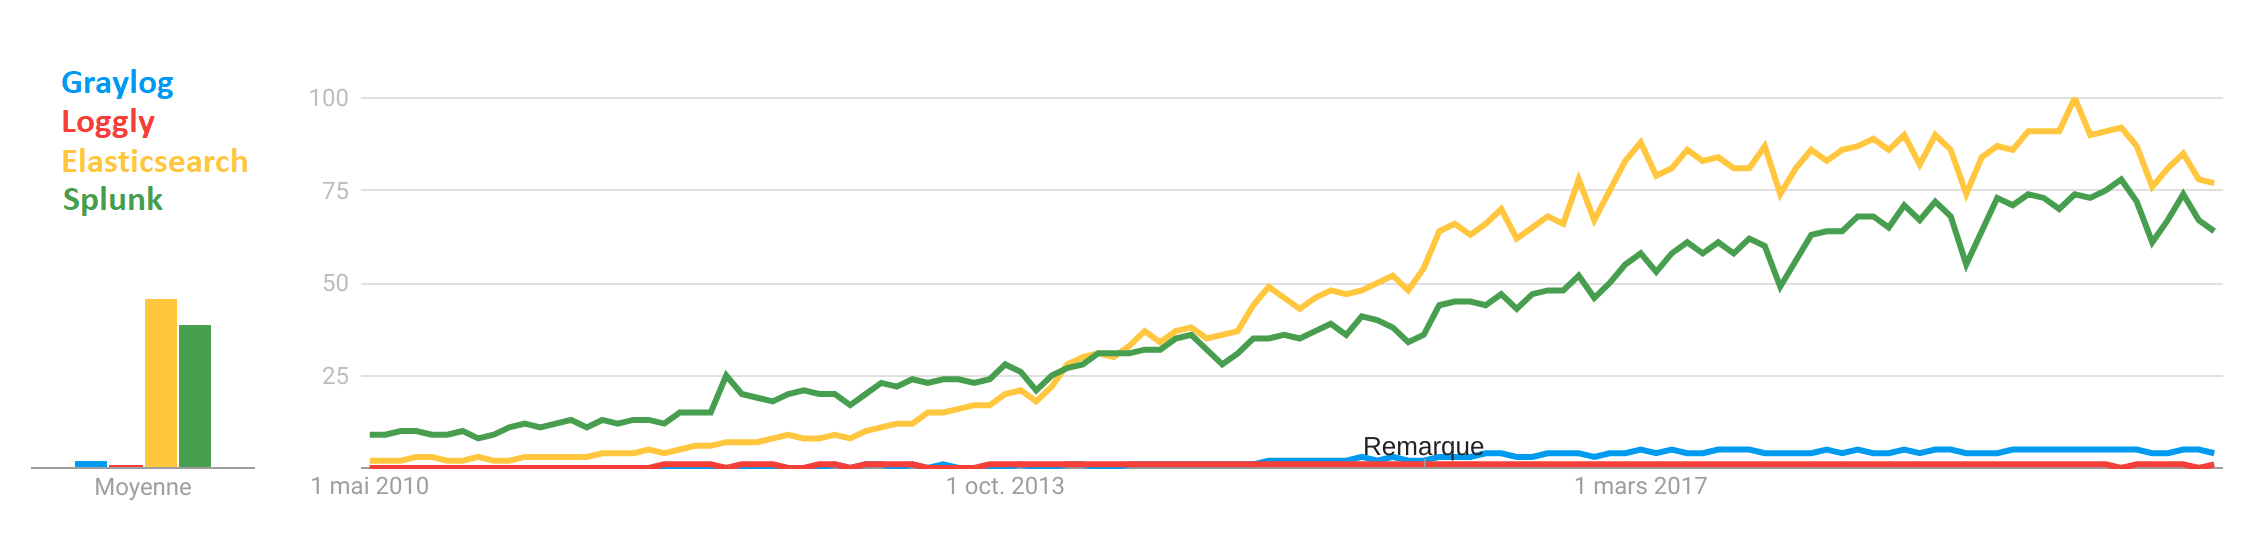
\includegraphics[width=18cm]{img/screenshots/Tendance_4.png}
    \caption{Courbes Google Trends des quatre systèmes}
    \label{f-Trends4Systemes}
\end{figure}

\begin{figure}[H]
    \centering
    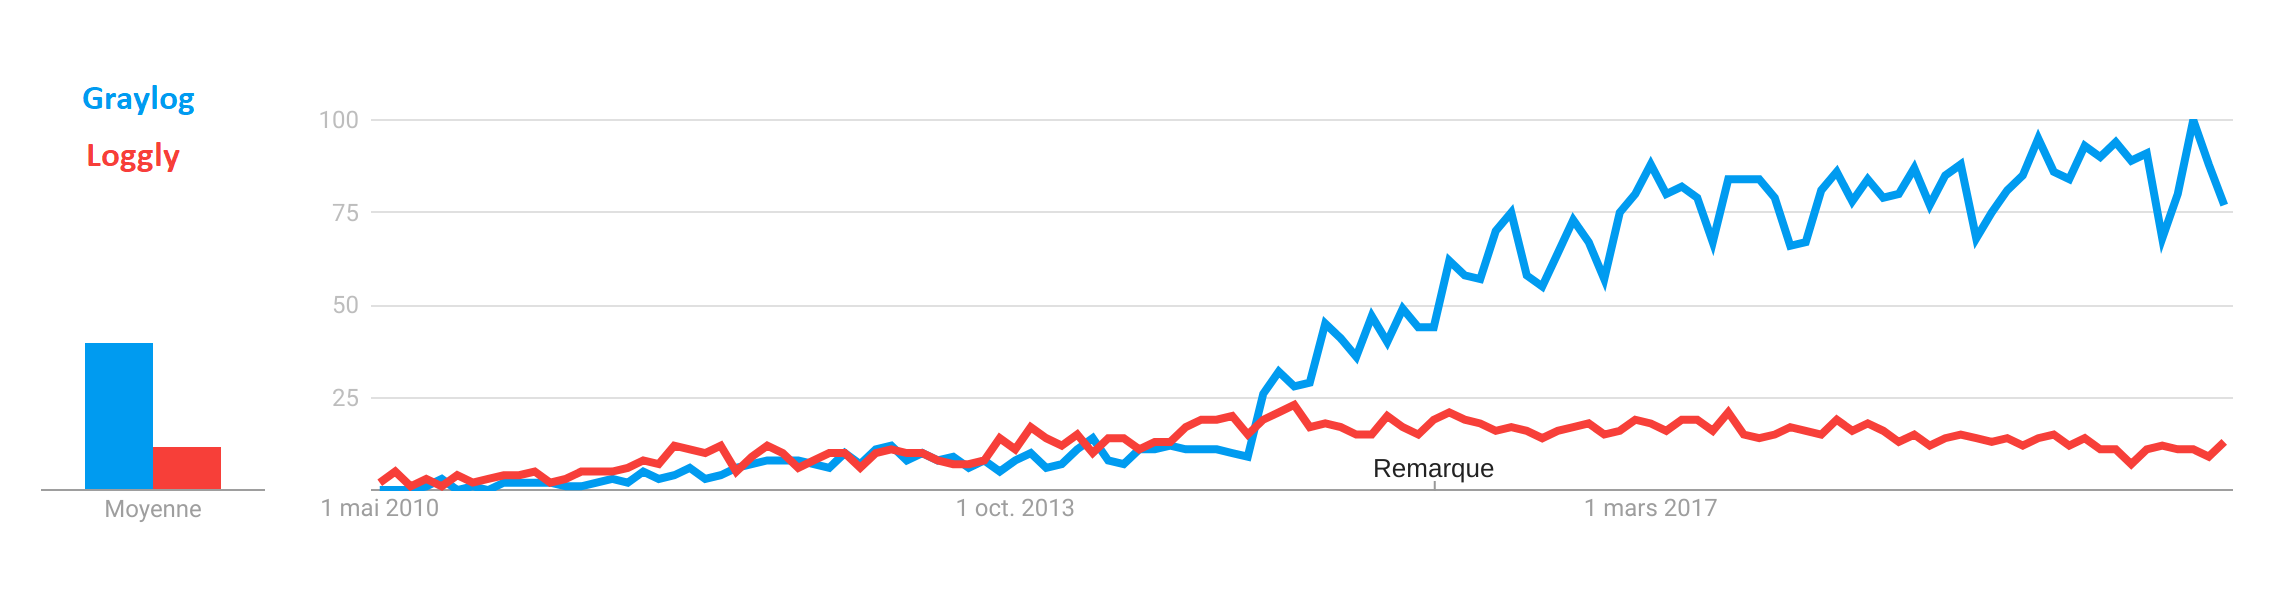
\includegraphics[width=18cm]{img/screenshots/Tendance_2.png}
    \caption{Courbes Google Trends de Graylog et Loggly}
    \label{f-Trends2Systemes}
\end{figure}

La Suite Elastic contenant 4 logiciels séparés, le choix ici a été d'inclure uniquement \og Elasticsearch \fg, car c'est la plus connue des quatre applications, et que les résultats sont meilleurs qu'avec le terme \og Elastic Suite \fg (il faut également savoir que la suite à changé de nom en 2016, passant de \og ELK Stack \fg à \og Elastic Stack \fg, ce qui ne favorise pas la recherche dans Google Trends).

\textbf{Conclusion} \\
On distingue deux groupes dans cette analyse : Elasticsearch et Splunk d'un côté, Graylog et Loggly de l'autre. Le premier est très populaire et en croissance, alors que le deuxième ne que peu tendance, et Loggly n'est pas en croissance. Au sein même du groupe Graylog-Loggly, on peut encore constater une grande différence, Graylog étant beaucoup plus recherché sur Google que Loggly. On peut donc affirmer que la Suite Elastic est le système le plus populaire, devant Splunk. Loin derrière vient Graylog et encore plus loin, on trouve Loggly.

\subsection{Tests réels et prise en main des logiciels}

Plusieurs tests ont été effectués afin de pouvoir effectuer une comparaison de ces systèmes. Comme la plupart de ces tests obligent une prise en main concrète des logiciels, ceux-ci ont également permis d'avoir une idée de la facilité d'utilisation, de la flexibilité ainsi que de l'utilisabilité ( \og user-friendliness \fg) des systèmes.

Voici les versions des logicielles utilisées pour effectuer ces tests :

\begin{itemize}
    \item Elastic Stack
    \subitem Elasticsearch 7.6.2
    \subitem Filebeat 7.6.2
    \subitem Logstash 7.6.2
    \subitem Kibana 7.6.2
    \item Graylog
    \subitem Graylog 3.2.4-1 (Virtual Appliance)
    \subitem Filebeat 7.6.2
    \item Splunk
    \subitem Splunk 8.0.2.1
    \subitem Splunk Universal Forwarder 8.0.2.1
    \item Loggly
    \subitem Loggly Lite (Cloud)
\end{itemize}

\subsubsection{Test de débit d'ingestion de log}

Le premier test de cette comparaison consiste en un test de débit. Cela permet d'avoir une première idée de la performance des applications.

\textbf{Conditions de tests} \\
\begin{itemize}
    \item Chargement d'un fichier de logs.
    \subitem Le fichier contient 98'305 logs identiques.
    \subitem Log : 2020-02-27 09:06:24.596 INFO  o.s.s.c.ThreadPoolTaskScheduler -> Shutting down ExecutorService 'taskScheduler'
    \item On effectue un test d'ingestion simple (on stocke le log brut).
    \item On effectue un test d'ingestion avec filtre (on parse les différentes parties du log).
    \subitem Date et heure : 2020-02-27 09:06:24.596
    \subitem Niveau du log : INFO
    \subitem Classe Java : o.s.s.c.ThreadPoolTaskScheduler
    \subitem Message : Shutting down ExecutorService 'taskScheduler'
    \item Le résultat est un débit exprimé en EPS (Event Per Second), qui correspond aux nombres de logs que le système aura pu ingéré en une seconde.
\end{itemize}

La table \ref{t-testIngestion} montre \textbf{les résultats} des tests d'ingestion.

\centering
\begin{table}[H]
\centering
\begin{tabular}{ |p{3cm}|p{3cm}|p{3cm}|p{3cm}|p{3cm}|  }
    \hline
    & Elastic Stack & Graylog & Splunk & Loggly \\
    \hline
    Sans filtrage & 4'898 & 14'044 & - & 46'295 (\textasteriskcentered) \\
    \hline
    Avec filtrage & 9'181 & 7'868 & 2'628 & -\\
    \hline
\end{tabular}
\caption{Résultats des tests de débit d'ingestion}
\label{t-testIngestion}
\end{table}
\justify

(*) Loggly n'acceptant que des fichiers de taille inférieure à 5 MB, le fichier à été réduit à 3'999 logs.

Splunk favorise l'extraction d'informations (parsing) après avoir stocké les logs dans le système. Il est donc compliqué d'ajouter un filtrage avant le stockage et ça n'a donc pas été réalisé. Par contre, Splunk effectue automatiquement une extraction de la date des logs. Son débit à donc été classé dans la catégorie \og avec filtrage \fg.
Loggly ayant été écarté assez tôt de l'évaluation, la partie \og avec filtrage \fg n'a pas été testée. \\

\textbf{Conclusion} \\
Sans filtrage, on constate que Graylog possède un débit supérieur à Elastic Stack. Loggly n'acceptant pas des fichiers de grande taille, il est difficilement comparable. Avec filtrage, étonnemment, la Suite Elastic gagne en débit. Elle possède donc un meilleur débit que Graylog et Splunk.
Après ce test, outre les résultats comptables, il se dessine surtout une tendance vers Graylog et Elastic Stack, car ces deux systèmes sont plus \og ouvert \fg que les autres. Il n'y a pas eu de difficultés particulières lors de l'utilisation, pas de contraintes comme la taille du fichier ou encore le moment du filtrage au sein du pipeline.

\subsubsection{Test d'ingestion d'une grande quantité de logs}

Ce test a pour but de mettre en évidence les limites de certains systèmes lors de l'ingestion de gros fichier de logs. Il permet également d'avoir une brève vue sur la constance du débit mesuré lors du test précédent.

\textbf{Conditions de tests} \\
\begin{itemize}
    \item Chargement d'un fichier de logs.
    \subitem Le fichier contient 999'999 logs identiques.
    \subitem Log : 2020-02-27 09:06:24.596 INFO o.s.s.c.ThreadPoolTaskScheduler -> Shutting down ExecutorService ’taskScheduler’
    \item On n'effectue aucun traitement sur le log.
    \item Le résultat est soit une limite supérieure, soit \og > 1'000'000 \fg
\end{itemize}

La table \ref{t-testGrandeIngestion} montre \textbf{les résultats} du test d'ingestion d'une grande quantité de logs.

\centering
\begin{table}[H]
\centering
\begin{tabular}{ |p{3cm}|p{3cm}|p{3cm}|p{3cm}|p{3cm}|  }
    \hline
    Elastic Stack & Graylog & Splunk & Loggly \\
    \hline
    > 1'000'000 & > 1'000'000 & > 1'000'000 & \textasciitilde 4'000 (5 MB) \\
    \hline
\end{tabular}
\caption{Résultats des tests d'ingestion de grande quantité de logs}
\label{t-testGrandeIngestion}
\end{table}
\justify

\textbf{Conclusion} \\
Ce test permet simplement de montrer que les systèmes travaillant avec un agent, soit selon la méthode PUSH, n'ont pas de problème de taille de fichier, car l'agent lit et envoie les logs au fur et à mesure. Loggly est le seul ici utilisant la méthode PULL. Au niveau des débits, ceux d'Elastic Stack et Graylog ont été divisé par 2, alors que celui de Splunk est resté stable. Pour Loggly, il n'y a pas eu de différence, étant donné qu'il est limité en taille de fichier.


\subsubsection{Test de consommation CPU}

Ce test-ci a pour but de pouvoir comparer les systèmes de gestion de logs Elastic Stack et Graylog en terme de performance.

\textbf{Conditions de test} \\
\begin{itemize}
    \item Chargement du même fichier de log que pour le test de débit.
    \item L'utilisation du CPU sera réduite au minimum hors système à tester.
    \item Ordinateur de test : ASUS UX360UAK
    \item Processeur : Intel Core i7-7500U CPU @ 2.70GHz x 4
    \item Lors de la réception, l'agent Filebeat se situera sur une autre machine.
\end{itemize}

\textbf{Résultats} \\
La figure \ref{f-ElasticCPU} montre la consommation CPU et l'historique du trafic réseau lors de la réception des logs. La figure \ref{f-GraylogCPU} montre les mêmes informations, mais pour le système Graylog. Enfin, la figure \ref{f-FilebeatCPU} montre ces informations-ci avec l'agent Filebeat.

\begin{figure}[H]
    \centering
    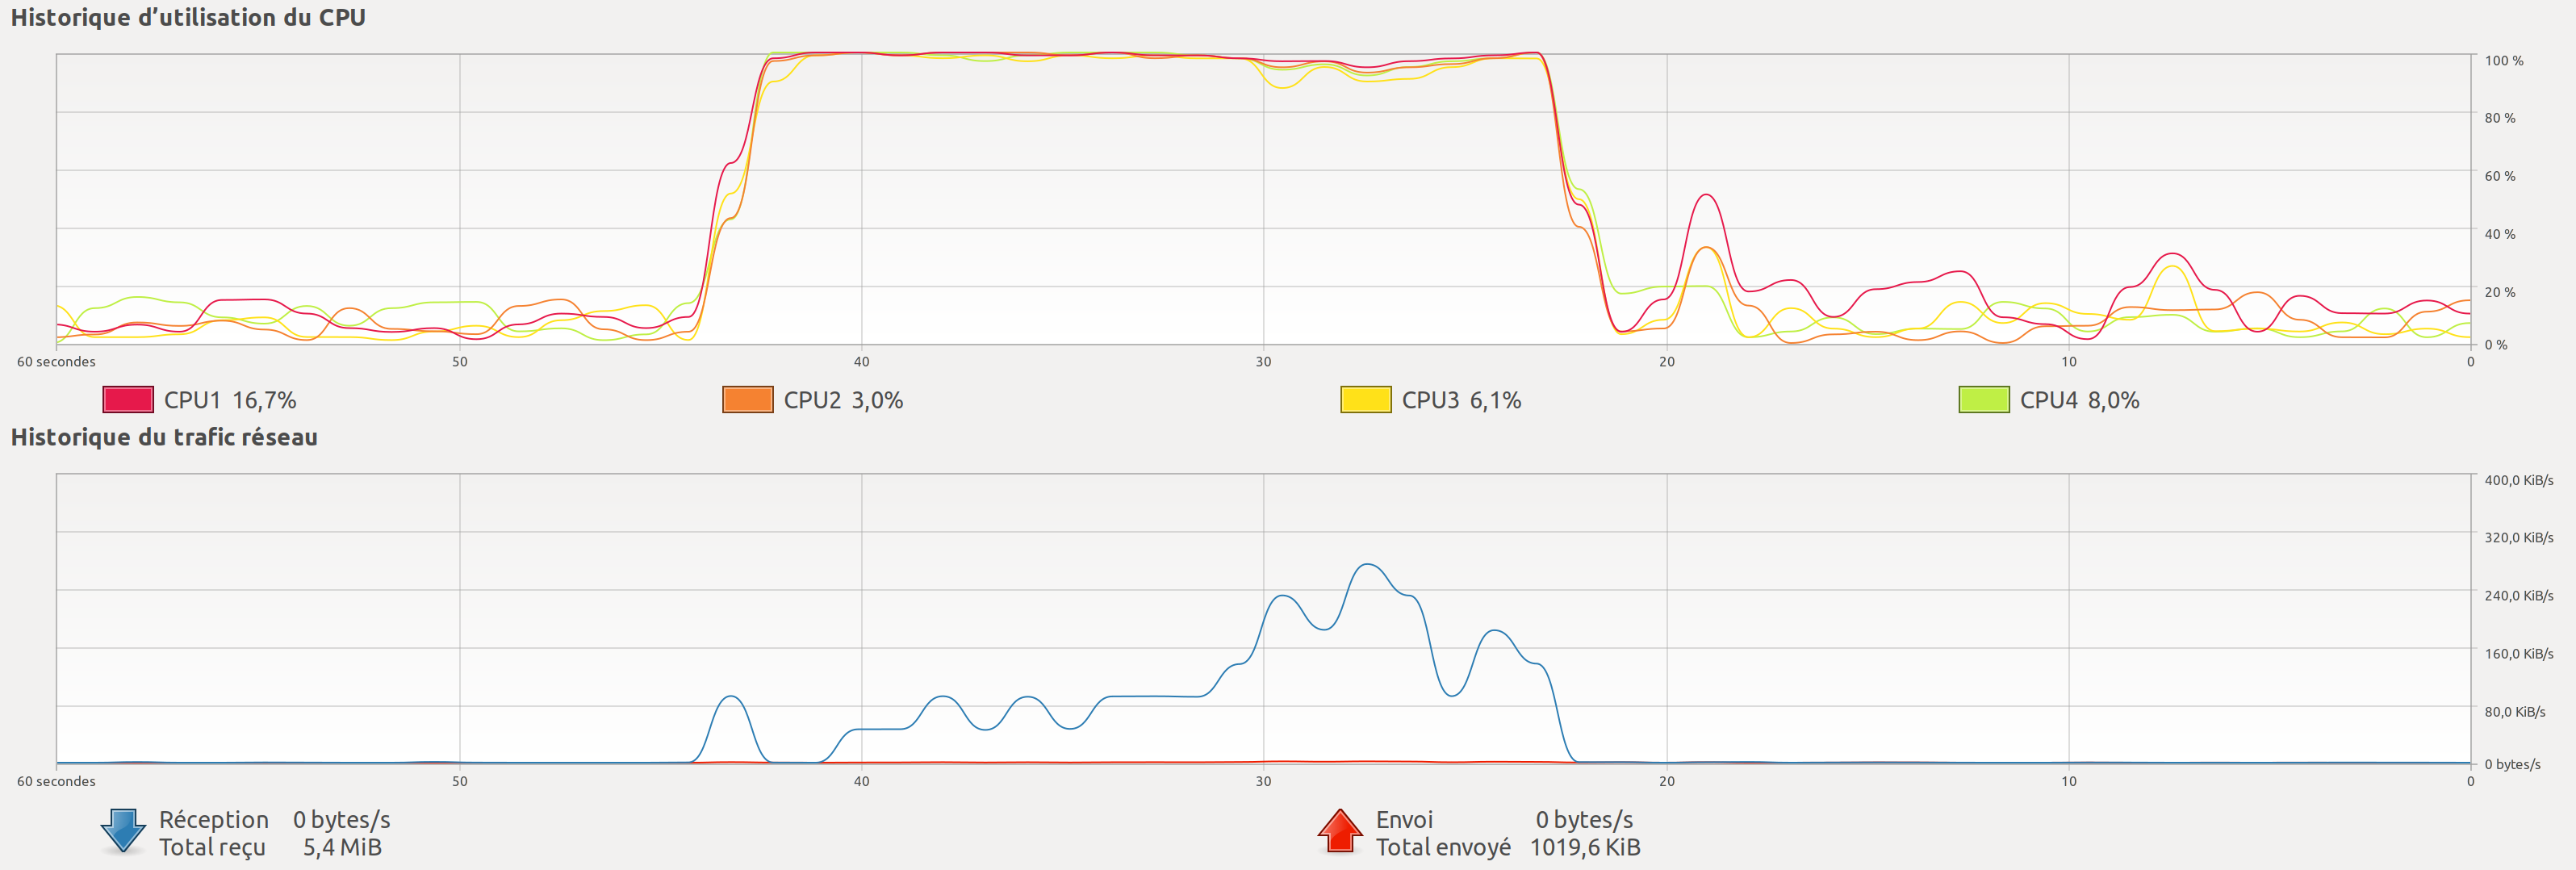
\includegraphics[width=18cm]{img/screenshots/Elastic_CPU_MEM_Receive_modified.png}
    \caption{Consommation CPU Elastic Stack}
    \label{f-ElasticCPU}
\end{figure}

\begin{figure}[H]
    \centering
    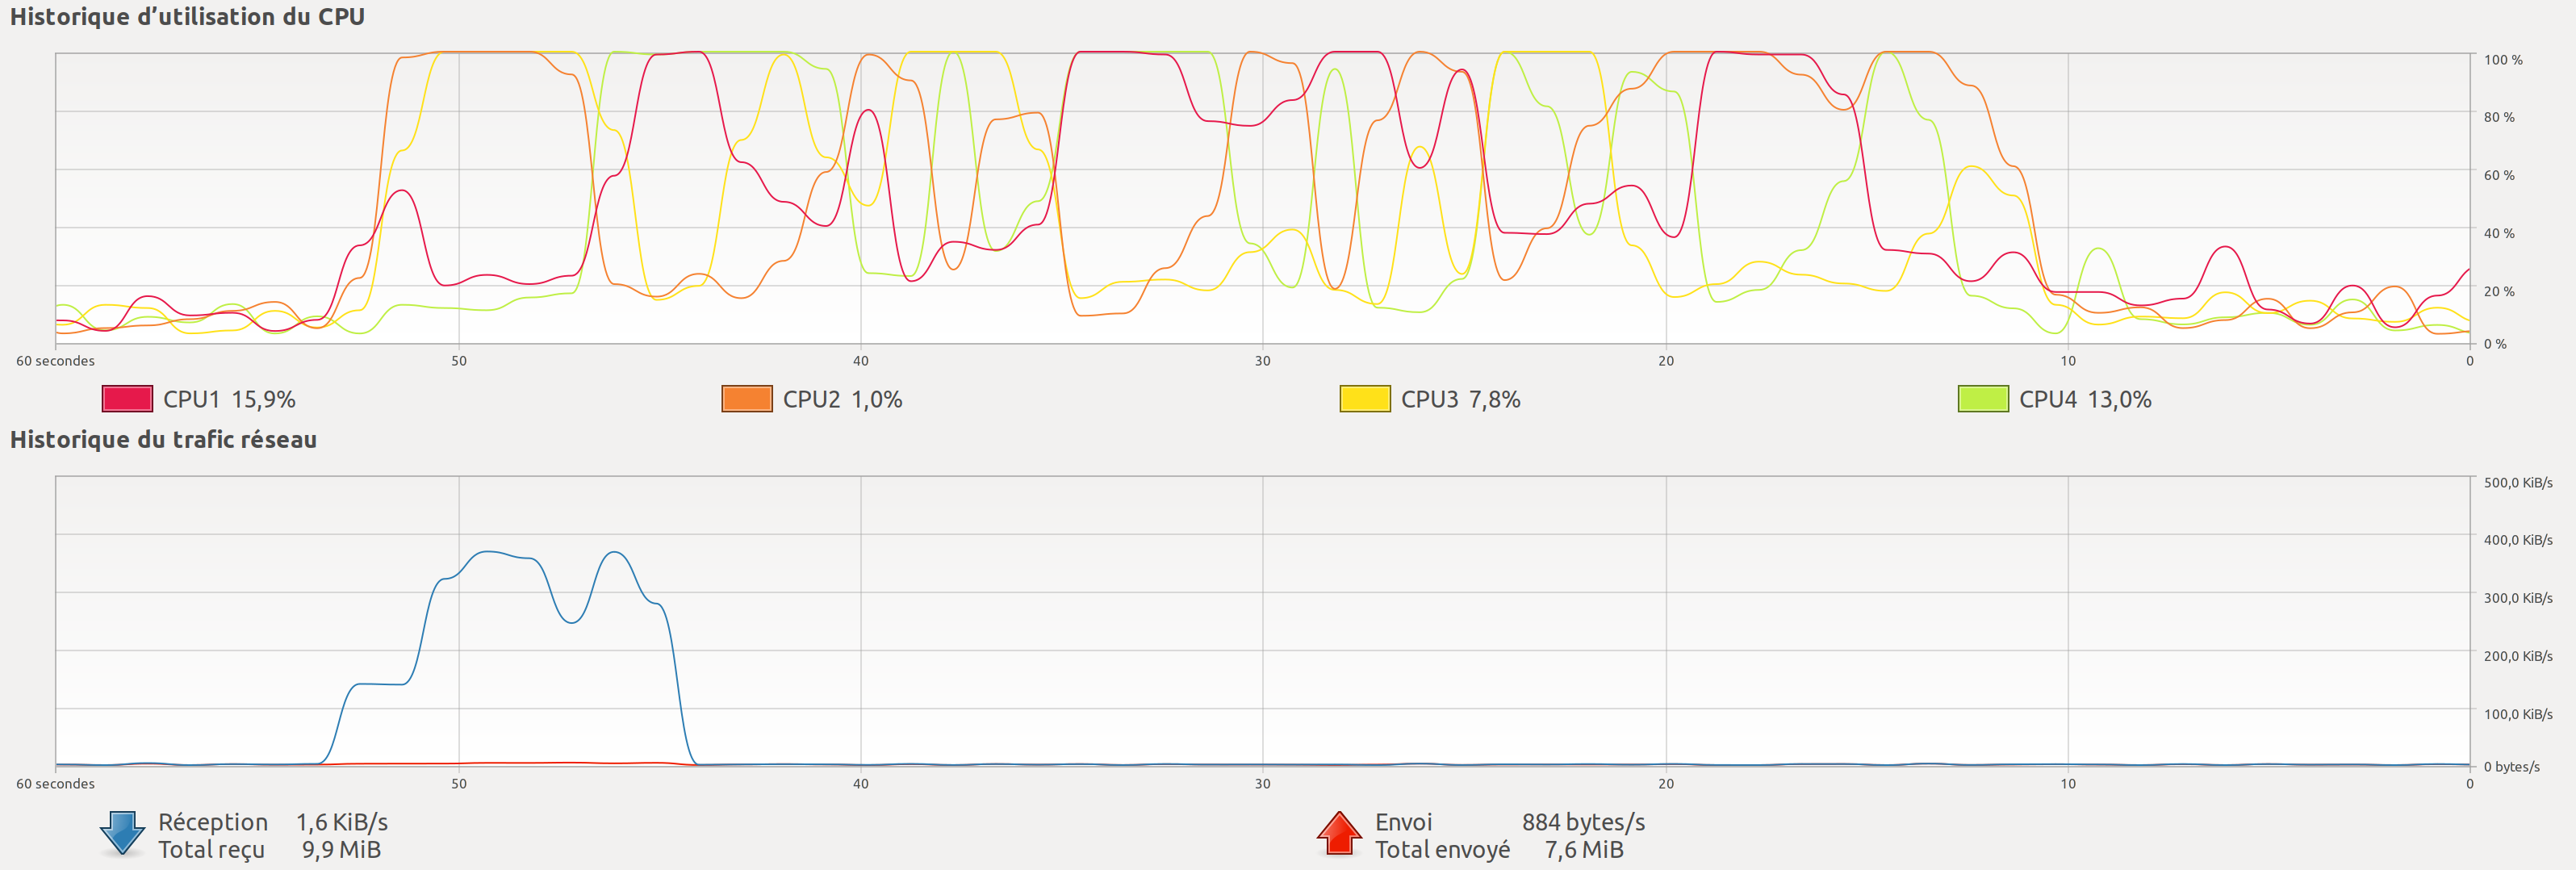
\includegraphics[width=18cm]{img/screenshots/Graylog_CPU_MEM_Receive_modified.png}
    \caption{Consommation CPU Graylog}
    \label{f-GraylogCPU}
\end{figure}

\begin{figure}[H]
    \centering
    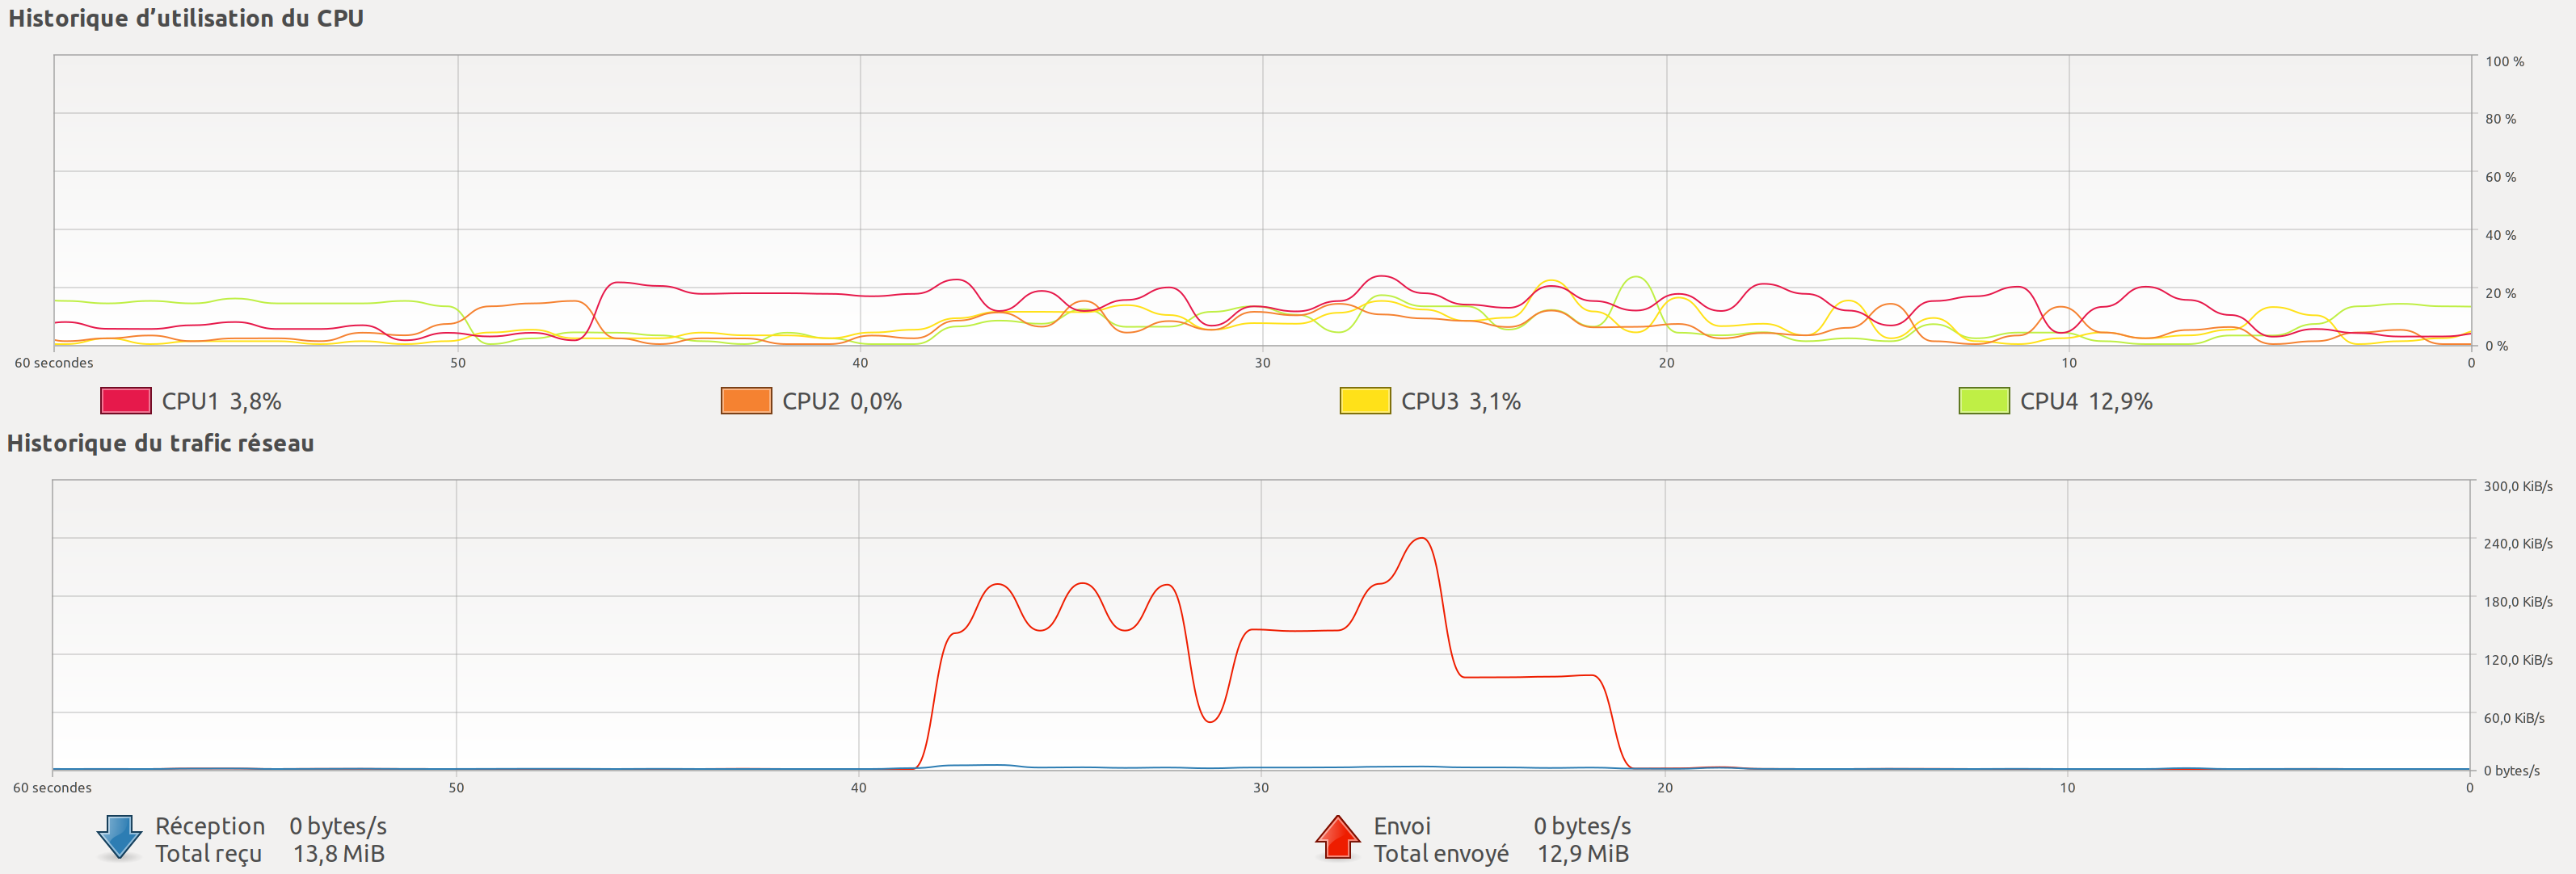
\includegraphics[width=18cm]{img/screenshots/Filebeat_send_modified.png}
    \caption{Consommation CPU Filebeat}
    \label{f-FilebeatCPU}
\end{figure}

\textbf{Conclusion} \\
Premièrement, on constate que l'agent Filebeat est un agent très léger puisque son action ne se fait quasiment pas ressentir sur le taux d'utilisation du CPU. Pour ce qui est du taux d'utilisation CPU par la Suite Elastic, on remarque que lors de la réception et le stockage des logs, tous les CPUs tournaient à 100\% de leur capacité, et la charge dure environ 25 secondes. Pour Graylog, les CPUs ne sont pas autant sollicité, ou du moins pas tous en même temps. Ils varient entre 20\% et 100\% et la distribution est plutôt égale entre les CPUs. On peut donc estimer un taux d'utilisation moyen à 60-70\%. La charge dure cette fois-ci environ 45 sec. À noter que Graylog ingère les logs en env. 7 secondes, puis travaille encore pendant env. 35 secondes, alors que la Suite Elastic fait tout en même temps. On peut constater ceci grâce à la courbe de l'historique du trafic réseau.

\subsection{Conclusion de l'évaluation}
\subsubsection{Analyse théorique des systèmes}
Au niveau fonctionnel, les quatre systèmes de gestion de logs ne se différencient pas énormément. Ils suivent à peu près tous le même schéma et permettent tous de faire les mêmes actions (reporting, alerting, analyse, etc.). Loggly est légèrement différent dans le sens où son approche de collecte de log par défaut est maximaliste (approche PULL). Il met en effet un endpoint à disposition, sur lequel on peut envoyer des données. Il s'agit la d'une différence mineure car bien que les autres systèmes privilégient et facilitent l'approche minimaliste, il est également possible de configurer un endpoint semblable pour les systèmes Elastic Stack, Graylog et Splunk.
Pour ce qui est du non-fonctionnel, il y a quelques points où les systèmes se démarquent. Premièrement, Loggly de SolarWinds est uniquement disponible dans une version Cloud. La Suite Elastic et Splunk sont eux disponibles tant dans une version Cloud que dans une version sur site. Graylog lui est uniquement disponible dans une version locale. Il y a également l'architecture des systèmes. La Suite Elastic est formée de 3 applications indépendantes, et en utilise une 4\ts{ème} pour l'agent Beat. Graylog est composé d'un système, et utilise des agents ne lui appartenant pas, comme Beat. Splunk suit la même architecture que Graylog, mais possède son propre agent, le Splunk Forwarder. Et Loggly est une infrastructure cloud sans agent.
Reste la comparaison de la popularité des applications. Celle-ci a montré une nette avance pour Splunk et Elastic Stack, devant Graylog, puis Loggly qui est vraiment peu populaire. \\
Globalement, l'analyse théorique des systèmes de gestion de logs ne permet pas de faire un choix concret sur un système ou un autre pour la réalisation d'une solution destinée au système GridEye. Elle permettrait tout au plus de se détacher de Loggly, qui n'est vraiment pas recommandable du point de vue de sa courbe de tendance.
\subsubsection{Analyse pratique des systèmes}
Le but des tests réels était de pouvoir confronter les systèmes de gestion de log au niveau de leur performance, et également de réaliser une prise en main des différents logiciels, avec tout ce que cela implique (installation, configuration, etc.). Cette deuxième partie avait également pour but d'évaluer l'utilisabilité des divers systèmes.
Au niveau des performances, on a pu voir que le système Graylog et Elastic Stack se distinguaient légèrement avec un meilleur débit d'ingestion. Que tous les systèmes, excepté Loggly, pouvaient, grâce à leur approche minimaliste, recevoir des grandes quantités de logs.\\
À ce point-ci de l'évaluation, un premier bilan de l'\og user-friendliness \fg des systèmes à également pu être tiré :
\begin{itemize}
    \item SolarWinds Loggly est relativement simple d'utilisation. Sa caractéristique Cloud facilite également l'installation (il n'y en a pas, il suffit de se créer un compte et nous recevons un lien vers notre version d'essai).
    \item Graylog est un système ayant une interface plutôt complète et efficace. L'interface graphique permet directement de configurer le système de manière simple (elle permet d'ajouter des règles d'extraction d'informations dans les logs, de configurer les entrées ouvert aux agents, etc.).
    \item Elastic Stack est une \og suite \fg de logiciels, ce qui la rend très ouverte. On peut en effet choisir d'utiliser ces software de base, mais également utiliser d'autres applications. Par exemple, on peu prendre un agent de la famille Beat, mais on pourrait aussi choisir un agent Prometheus. Chaque logiciel est configurable via des fichiers de configuration. On peut également choisir d'utiliser les 4 logiciels, ou pas. Par exemple enlever Logstash si l'on a pas besoin de ces filtres. Cette ouverture le rend agréable à utiliser.
    \item Splunk est comparable à Graylog et Elastic Stack dans tous les tests, mais l'expérience utilisateur est de son côté moins bonne. Le système est plus une sorte de \og boîte noire \fg dans laquelle il n'est pas possible de tout configurer. L'extraction des informations des logs n'a par exemple pas pu avoir lieu avant l'indexage, car le système est prévu pour le faire après.
\end{itemize}
Avec ces premiers tests, nous avons déjà pu écarter la solution SolarWinds Loggly, qui ne correspondait pas aux attentes et dont les contraintes liées au Cloud ne sont pas souhaitées. Splunk n'est également pas recommandé à cause de son manque d'ouverture.
Ensuite, il y a encore eu le test d'utilisation du CPU entre la Suite Elastic et Graylog. Avec celui-ci, on pourrait donner un très léger avantage à Graylog.

\subsubsection{Recommandation}
En conclusion, il est difficile de faire un choix entre les deux systèmes Graylog et la Suite Elastic. Mais de part sa très grande popularité, amenant son lot de réponse dans les forums et autre article permettant d'accélérer le développement d'un logiciel, ainsi que de son caractère très ouvert lié à son \og architecture suite \fg, la \textbf{Suite Elastic} est le meilleur choix dans l'optique de mise en place d'une solution de gestion de logs pour l'infrastructure GridEye.

\newpage

\section{Implémentation du cas d'utilisation}

\subsection{Installation de la Suite Elastic}

Lors de l'installation de la Suite Elastic, il est important (et obligatoire) d'avoir la même version pour tous les composants. P. ex. dans le cas présent, la version 7.6.2 est utilisée. On aura donc Elasticsearch 7.6.2, Logstash 7.6.2, etc.
L'installation doit également suivre un ordre particulier :
\begin{enumerate}
    \item Elasticsearch
    \item Kibana
    \item Logstash
    \item Beats
\end{enumerate}
L'installation décrite ici est réalisée sur un système Ubuntu 20.04.

\subsubsection{Elasticsearch}
Téléchargement du paquet \verb,.deb, et de sa signature.
\begin{lstlisting}[language=bash]
wget https://artifacts.elastic.co/downloads/elasticsearch/elasticsearch-7.6.2-amd64.deb
wget https://artifacts.elastic.co/downloads/elasticsearch/elasticsearch-7.6.2-amd64.deb.sha512
\end{lstlisting}
Il faut contrôler la signature SHA du paquet téléchargé, en la comparant avec la somme de contrôle publique.
\begin{lstlisting}[language=bash]
shasum -a 512 -c elasticsearch-7.6.2-amd64.deb.sha512
\end{lstlisting}
La réponse doit être \verb,elasticsearch-7.6.2-amd64.deb: OK,, avec le bon numéro de version.
Il suffit enfin d'installer le paquet précédemment téléchargé.
\begin{lstlisting}[language=bash]
sudo dpkg -i elasticsearch-7.6.2-amd64.deb
\end{lstlisting}
Afin de tester si l'installation est réussie, il faut lancer Elasticsearch
\begin{lstlisting}[language=bash]
sudo -i service elasticsearch start
\end{lstlisting}
Une fois la commande exécutée, à l'aide d'un navigateur, le bon fonctionnement d'Elasticsearch est contrôlable à l'adresse \verb,localhost:9200,. Ou alors avec la commande \verb,curl, suivante :
\begin{lstlisting}[language=bash]
curl -X GET "localhost:9200/?pretty"
\end{lstlisting}

La figure \ref{f-elasticsearchInstalled} montre une installation complète et réussie.
\begin{figure}[H]
    \centering
    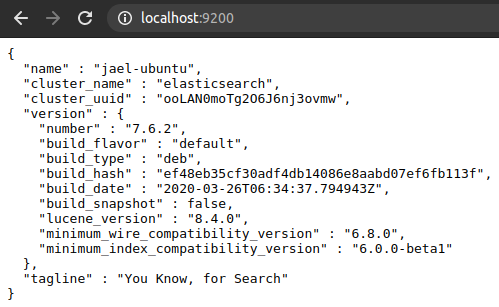
\includegraphics[width=9cm]{img/screenshots/elasticsearch_installed.png}
    \caption{Page d'accueil Elasticsearch}
    \label{f-elasticsearchInstalled}
\end{figure}
L'application s'arrête également grâce à la commande \verb,service,.
\begin{lstlisting}[language=bash]
sudo -i service elasticsearch stop
\end{lstlisting}

\subsubsection{Kibana}
Téléchargement du paquet \verb,.deb, et de sa signature.
\begin{lstlisting}[language=bash]
wget https://artifacts.elastic.co/downloads/kibana/kibana-7.6.2-amd64.deb
wget https://artifacts.elastic.co/downloads/kibana/kibana-7.6.2-amd64.deb.sha512
\end{lstlisting}
Il faut contrôler la signature SHA du paquet téléchargé, en la comparant avec la somme de contrôle publique.
\begin{lstlisting}[language=bash]
shasum -a 512 -c kibana-7.6.2-amd64.deb.sha512
\end{lstlisting}
La réponse doit être \verb,kibana-7.6.2-amd64.deb: OK,, avec le bon numéro de version.
Il suffit enfin d'installer le paquet précédemment téléchargé.
\begin{lstlisting}[language=bash]
sudo dpkg -i kibana-7.6.2-amd64.deb
\end{lstlisting}
Afin de tester si l'installation est réussie, il faut lancer Kibana
\begin{lstlisting}[language=bash]
sudo -i service kibana start
\end{lstlisting}
Une fois la commande exécutée, à l'aide d'un navigateur, le bon fonctionnement de Kibana est contrôlable à l'adresse \verb,localhost:5601,.

La figure \ref{f-kibanaInstalled} montre une installation complète et réussie.
\begin{figure}[H]
    \centering
    
\includegraphics[width=11cm]{img/screenshots/kibana_installed.png}
    \caption{Page d'accueil Kibana}
    \label{f-kibanaInstalled}
\end{figure}
L'application s'arrête également grâce à la commande \verb,service,.
\begin{lstlisting}[language=bash]
sudo -i service kibana stop
\end{lstlisting}

\subsubsection{Logstash}
Logstash nécessite la présence de Java sur son système. L'installation décrite ci-dessous fonctionne avec une version de Java open-source : \verb,OpenJDK,. Il est bien sûr possible d'utiliser la version Java officielle d'Oracle.

Il faut donc contrôler si Java est bien présent sur la machine.
\begin{lstlisting}[language=bash]
java -version
\end{lstlisting}
Sur un système avec Java installé, la réponse est de la forme suivante :
\begin{lstlisting}[language=bash]
openjdk version "11.0.7" 2020-04-14
OpenJDK Runtime Environment (build 11.0.7+10-post-Ubuntu-3ubuntu1)
OpenJDK 64-Bit Server VM (build 11.0.7+10-post-Ubuntu-3ubuntu1, mixed mode, sharing)
\end{lstlisting}

Tout d'abord, il faut télécharger et installer la clé PGP d'Elastic permettant de télécharger le paquet avec \verb,APT,.
\begin{lstlisting}[language=bash]
wget -qO - https://artifacts.elastic.co/GPG-KEY-elasticsearch | sudo apt-key add -
\end{lstlisting}
Il faut ensuite télécharger, si ce n'est pas déjà le cas sur la machine, installer le paquet \verb,apt-transport-https,.
\begin{lstlisting}[language=bash]
sudo apt-get install apt-transport-https
\end{lstlisting}
Il faut ensuite sauvegarder la définition du répertoire à \verb,/etc/apt/sources.list.d/elastic-7.x.list,.
\begin{lstlisting}[language=bash]
echo "deb https://artifacts.elastic.co/packages/7.x/apt stable main" | sudo tee -a /etc/apt/sources.list.d/elastic-7.x.list
\end{lstlisting}
Enfin, il faut télécharget et installer Logstash.
\begin{lstlisting}[language=bash]
sudo apt-get update && sudo apt-get install logstash
\end{lstlisting}
Il est possible de tester si Logstash a été correctement installé en le lançant. Cependant, il ne sera passera rien, car il n'est pas configuré. Toutefois, si le système ne renvoie pas d'erreur, c'est que Logstash a été correctement installé, en principe.
\begin{lstlisting}[language=bash]
sudo systemctl start logstash.service
\end{lstlisting}
Logstash s'arrête avec une commande similaire.
\begin{lstlisting}[language=bash]
sudo systemctl stop logstash.service
\end{lstlisting}

La partie \og serveur \fg est de la Suite Elastic est maintenant installée. Il reste encore à installer un agent Beat sur la machine générant les logs.

\subsubsection{Beat}
Il existe toute une panoplie d'agent de transfert léger dans la famille Beat. La liste des agents Beat existants est disponible sur le site d'Elastic. Il existe des Beat créés par Elastic, et également un grand nombre de Beat communautaires, créés, comme leur nom l'indique, par la communauté (p. ex. dockbeat pour Docker, Kafkabeat pour Kafka, etc.).
Comme le programme de simulation de l'infrastructure GridEye utilisé pour l'implémentation du cas d'utilisation stocke les logs générés dans un fichier, le descriptif d'installation de ce document se concentrera sur l'installation d'un agent de type \verb,Filebeat,.

Sur la machine générant les logs, il faut donc télécharger le paquet de \verb,Filebeat,.
\begin{lstlisting}[language=bash]
curl -L -O https://artifacts.elastic.co/downloads/beats/filebeat/filebeat-7.6.2-amd64.deb
\end{lstlisting}
Finalement, il faut installer le paquet téléchargé.
\begin{lstlisting}[language=bash]
sudo dpkg -i filebeat-7.6.2-amd64.deb
\end{lstlisting}

Comme pour Logstash, il est possible de tester si Filebeat a été correctement installé en le lançant. Cependant, il ne sera passera rien, car il n'est pas configuré. Toutefois, si le système ne renvoie pas d'erreur, c'est que Filebeat a été correctement installé, en principe.
\begin{lstlisting}[language=bash]
sudo service filebeat start
\end{lstlisting}
Filebeat s'arrête avec une commande similaire.
\begin{lstlisting}[language=bash]
sudo service filebeat stop
\end{lstlisting}

\newpage

\thispagestyle{empty}
\centering
\vspace{10cm}
{\huge ANNEXES}

\newpage

\appendix
\justify

\listoftables
\newpage

\listoffigures
\newpage

\section{Bibliographie}
\section{Détails des tests}

\subsection{Tests de débit d'ingestion}

Graylog (3.2.4 Virtual appliance) avec Filebeat :

Sans extractor (module de Graylog permettant le parsing des logs) :

Début du chargement : 10:09:17 \\
Fin du chargement : 10:09:24 \\
Temps de chargement : 7 secondes \\
Débit moyen : \textasciitilde 14'043,47 EPS \\

Avec extractor :

Début du chargement : 07:46:47.153 \\
Fin du chargement : 07:46:59.648 \\
Temps de chargement : 12.495 secondes \\
Débit moyen : \textasciitilde 7'867,55 EPS \\

Elastic Stack sans Logstash :

Début du chargement : 10:34:34.200 \\
Fin du chargement : 10:35:03.622 \\
Temps de chargement : 29.422 secondes \\
Débit moyen : \textasciitilde 3'341,21 EPS \\

Elastic Stack complet (sans filtrage du log) :

Début du chargement : 10:44:11.851 \\
Fin du chargement : 10:44:31.920 \\
Temps de chargement : 20.069 secondes \\
Débit moyen : \textasciitilde 4'898,35 EPS \\

Elastic Stack complet (avec filtrage du log) :

Début du chargement : 10:26:37.308 \\
Fin du chargement : 10:26:48.015 \\
Temps de chargement : 10.707 secondes \\
Débit moyen : \textasciitilde 9'181,38 EPS \\

Splunk :

Avec filtrage : \\
Donné (metrics.log de Splunk) : 2'628 EPS \\

Solarwinds Loggly avec endpoint bulk :
Avec Loggly, il est impossible de charger un fichier de plus de 5 MB. Il a donc été réduit à 39'999 lignes.

Début du chargement : 08:42:11.360 \\
Fin du chargement : 18:42:12.224 \\
Temps de chargement : 0.864 seconde \\
Débit moyen : \textasciitilde 46'295,14 EPS \\

\section{Journal de travail}


\subsection{Jeudi 13 février}
    Première réunion avec Nastaran, Jonathan et Pascal. Jonathan et Pascal ont expliqué leur vision du TB à travers une présentation, puis nous avons planifié le travail de Bachelor. Notamment les dates de fin d'évaluation (avec la présentation à DEPsys), et de fin de développement du use-case.
\subsection{Mercredi 19 février}
    Début du Travail de Bachelor. J'ai commencé par suivre un tuto afin de maîtriser les bases du langage \LaTeX, ce qui me sera utile pour tout ce qui est rédactionnel. Ensuite, j'ai commencé à revoir la présentation de Pascal afin de bien comprendre (notamment les technologies que je ne connais pas).
\subsection{Jeudi 20 février}
    J'ai regardé plusieurs vidéos qui présentent les différentes technologies que je dois évaluer.
\subsection{Mercredi 26 février}
    J'ai décidé de commencer à évaluer plus en profondeur Elasticsearch en premier, car Prometheus à comme contrainte de ne pas gérer les logs textuels, mais uniquement des métriques numériques. Cependant, d'après plusieurs lectures, je pense qu'il pourrait être intéressant de mixer les deux solutions. J'ai donc installé les outils de la suite ELK, et suivi des tutos plus concret en ce qui concerne Elasticsearch (insertion de donnée, recherches, etc.).
\subsection{Jeudi 27 février}
    Deuxième réunion avec Nastaran. Elle me propose de recentrer mes recherches sur la partie \og Log Analysis \fg, donc rechercher directement l'intégration de l'analyse de logs avec ELK par exemple. Après la réunion, j'ai donc continuer mes recherches dans ce sens et ai suivi la vidéo de elastic qui concerne l'analyse de logs.
\subsection{Mercredi 04 mars}
    J'ai commencé à écrire ce journal afin de mieux me rappeler de ce que j'ai fais, ainsi que d'être plus structuré. Je commence également à utiliser Zotero, qui permet d'enregistrer tous les liens que je trouve intéressant, ainsi que de créer une bibliographie. J'ai également décidé de m'intéresser à Graylog en plus de ELK.
\subsection{Jeudi 05 mars}
    J'ai exploré plus en profondeur les articles de type \og Elastic Stack versus Graylog \fg, et je vais donc inclure la stack \og Graylog server, MongoDB et Elasticsearch \fg dans le comparatif. Cette suite-là me semble très appropriée au traitement et à l'analyse de logs.
    J'ai été à la réunion avec Nastaran à 11h30. Suite à cette réunion, nous avons décidé qu'il fallait que je fasse une synthèse des mes recherches et que je la présente en quelques slides le jeudi 12 mars.
\subsection{Lundi 09 mars}
    J'ai commencé à faire la synthèse de mes recherches. Je vais donc la faire en 3 étapes :
    \begin{enumerate}
    \item Choix des critères d'évaluations
        \begin{enumerate}
            \item Selon des recherches au sujet des caractéristiques d'un \og Log Management Tool \fg
        \end{enumerate}
    \item Choix des outils à évaluer
        \begin{enumerate}
                \item Pour cette étape, je vais consulter plusieurs classements de système de gestion de logs et choisir ceux qui sont le plus souvent cités. Je vais probablement en prendre 5 ou 6.
        \end{enumerate}
    \item Synthèse et rédaction des slides
    \end{enumerate}
    Ce lundi, j'ai défini les critères d'évaluation, selon les demandes de DEPsys ainsi que les critères lu lors de mes recherches.
\subsection{Mercredi 11 mars}
    J'ai fais un tableau pour le choix des outils à tester. J'ai donc effectué un classement selon 4 tops de système de gestion de logs.
    J'ai également commencé l'évaluation à proprement parler, en particulier sur Elastic Stack et Graylog. J'ai également eu un problème de stockage de la base de donnée Zotero et j'ai perdu toute ma bibliographie.
\subsection{Jeudi 12 mars}
    J'ai continué l'évaluation avec Loggly, j'ai créé la présentation de synthèse pour la réunion avec Nastaran, puis je l'ai présentée.
\subsection{Mercredi 18 mars}
    J'ai remis en place Zotero, cette fois avec un synchronisation en ligne de ma bibliographie. J'ai analysé les différents systèmes de gestion de logs que j'hésitais à inclure dans l'évaluation. J'ai donc écarté ManageEngine EventLog Analyzer pour sa popularité vraiment faible et son manque de documentation, et PRTG Network Monitor, qui est très axé sur l'analyse d'un réseau, comme son nom l'indique. Je vais donc évaluer Splunk.
\subsection{Jeudi 19 mars}
    J'ai fais l'évaluation de Splunk. J'ai également eu la réunion hebdomadaire avec Nastaran.
\subsection{Samedi 21 mars}
    J'ai reformaté mon rapport avec le template \LaTeX écrit par Mateo Tutic. J'ai également développé la partie Choix des différents systèmes à évaluer.
\subsection{Dimanche 22 mars}
    J'ai continué la partie Choix des différents systèmes à évaluer. J'ai également télécharger la suite Elastic et testé avec les logs systèmes de Ubuntu. Cela fonctionne normalement.
\subsection{Lundi 23 mars}
    J'ai mis en place les systèmes de gestion de logs Elastic Stack, Graylog, Splunk et Loggly. J'ai testé (en insérant des logs et regardant le débit) les 3 premiers. Encore quelques problèmes pour Loggly (pour l'instant, il sauvegarde 1 log avec n lignes dans le message plutôt que n logs avec 1 ligne). J'ai également terminé les tableaux récapitulatif de l'évaluation de chaque système.
\subsection{Mardi 24 mars}
    J'ai terminé les tests d'ingestions de logs pour les 4 systèmes. J'ai commencé à faire mes slides pour la présentation du 25 mars.
\subsection{Mercredi 25 mars}
    J'ai terminé les slides de la présentation. J'ai fais la présentation du travail de Bachelor à l'entreprise DEPsys. S'en est suivi une discussion avec Pascal, Jonathan, Nastaran et moi au sujet de la suite de l'évaluation de mon TB, puis un ajustement du cas d'utilisation à implémenter fourni par Pascal.
\subsection{Jeudi 26 mars}
    J'ai commencé à refaire des tests d'ingestion de log. Cette fois-ci avec tout le pipeline. Je commence avec Elastic Suite, en y intégrant logstash afin qu'il filtre les données.
\subsection{Mercredi 01 avril}
    J'ai continué les tests d'ingestion avec Elastic Suite et rencontré beaucoup de problème. J'arrive à faire fonctionner un pipeline Logstash-Elasticsearch-Kibana, et un pipeline Filebeat-Elasticsearch-Kibana, mais pas un contenant les 4 logiciels de la suite.
\subsection{Jeudi 02 avril}
    J'ai continué les tests en tentant plusieurs tutoriaux trouvé sur internet. Mais je rencontre toujours des problèmes. Ils sont probablement liés à la communication entre Filebeat et Logstash. J'ai également suivi les tuto officiels de la Suite Elastic, mais ça n'a pas fonctionné non plus. Ceci est peut-être dû à mes fichiers de configurations des logiciels Filebeat et Logstash. J'ai ensuite eu une réunion avec Nastaran.
\subsection{Mercredi 08 avril}
    J'ai continué les tests d'ingestion. En suivant les guides du site d'elastic, j'ai remarqué qu'il y avait toute une section expliquant l'utilisation de la Suite avec Docker. Je me suis dit qu'il y avait plus de chance que cela fonctionne étant donné l'uniformité que propose Docker. Malheureusement, j'ai toujours les mêmes problèmes. Même en prenant un git public sensé fonctionner. Je me dit alors que le problème vient peut-être de mes fichiers de logs de tests (ils contiennent le même log multiplié n fois).
\subsection{Jeudi 09 avril}
    Je suis repassé sur une version non dockerisée de la suite Elastic. J'ai téléchargé un fichier de log d'un serveur Apache afin de tester la Suite avec un fichier de log réel, et fait d'autres modifications, notamment sur les fichiers de configuration (j'ai créé la partie \og filtrage \fg de Logstash avec un site internet permettant de créer ces filtres de manière incrémentale). Et ça à fonctionné. J'ai ensuite eu la réunion avec Nastaran.
\subsection{Lundi 13 avril}
    J'ai effectué les tests de performances avec filtrage de la Suite Elastic. Après ceci, je me suis lancé dans les tests avec filtrage de Graylog. Cette fois-ci, ce n'est pas avec un logiciel intermédiaire comme Logstash, mais avec une fonctionnalité intégrée à Graylog : les Graylog Extractors.
\subsection{Mercredi 15 avril}
    J'ai commencé à cherché une façon d'effectuer le filtrage avec le système de gestion de logs Splunk. Malheureusement, j'ai l'impression que cela va être plus compliqué car Splunk favorise l'extraction des informations après l'indexage. Je vais encore chercher une journée, et si ce n'est pas concluant, je passerai outre.
\subsection{Jeudi 16 avril}
    J'ai tenté d'effectuer l'extraction d'informations dans les logs durant la phase de "parsing" du pipeline de Splunk. J'ai vu qu'il devait être possible de le faire en modifiant des fichiers de configuration dans le répertoire de Splunk, mais cela n'a pas fonctionné.
\subsection{Lundi 20 avril}
    J'ai rédigé les résultats des tests d'ingestion. J'ai ensuite commencé à étudié les manières de faire des tests de consommation CPU. Sachant qu'avec Amazon Web Service (AWS), comme je l'avais vu quelques semaines plus tôt dans un cours de Cloud Computing, il est possible de monitorer différentes métriques d'une instance, entre autres l'utilisation du CPU, je me suis lancé dans une installation de la Suite Elastic sur une instance t2.micro d'AWS. Malheureusement, ces instances sont trop petites et ne supportent pas simplement Elasticsearch. Ne voulant pas payer pour des instances plus grosses, je me suis rabattu sur la solution locale. Je vais donc simplement stopper le maximum de processus et monitorer l'utilisation de mon CPU avec l'outil natif d'Ubuntu. Je dois aussi installer Filebeat et Graylog sur un autre ordinateur afin de pouvoir effectué ces tests (dans la réalité, le serveur et le client ne seront pas sur la même machine).
\subsection{Mercredi 22 avril}
    J'ai effectué les tests de consommation CPU de la Suite Elastic, de Graylog, ainsi que de Filebeat. J'ai ensuite commencé à rédiger la synthèse de ces tests.
\subsection{Jeudi 23 avril}
    J'ai continué la rédaction, j'ai ajouté le test d'ingestion d'un grand nombre de logs, la comparaison de popularité.
\subsection{Vendredi 24 avril}
    J'ai rédigé le cahier des charges, puis ai eu une réunion avec Nastaran. Nous avons discuté du cahier des charges, des améliorations à y apporter. Ensuite, nous avons un peu regarder l'état du rapport actuel. Il faut entre autre pense a y ajouter les références (tableaux, image, bibliographie). Nous avons ensuite convenu de fixer une réunion avec Jonathan et Pascal afin de leur présenter les résultats de l'évaluation. J'ai donc fixé cette réunion à jeudi 30 avril.
\subsection{Mercredi 29 avril}
    J'ai modifié le rapport pour y ajouter les références sur les tableaux et sur les figures. J'ai également amélioré les annexes avec la table des tableaux et la table des figures. J'ai également commencé la conclusion finale de l'évaluation, en rédigeant le paragraphe concernant l'analyse théorique.
\subsection{Jeudi 30 avril}
    J'ai continué le rapport. J'y ai ajouté une conclusion finale à l'évaluation. J'ai ensuite eu une réunion avec Pascal, Jonathan et Nastaran. Je leur ai présenté les résultats de mon évaluation et nous avons convenu ensemble d'effectuer l'implémentation du cas d'utilisation avec le système Elastic Stack.
\subsection{Mercredi 6 mai}
    J'ai pris en main le programme de Jonathan qui simule l'infrastructure GridEye de façon minimale. Je l'ai modifié légérement pour qu'il stocke les logs dans un fichier, plutôt que de les afficher dans la console. J'ai ensuite commencé à rédiger la partie implémentation du cas d'utilisation dans le rapport, tout en testant les commandes que je met dans le rapport sur une installation neuve d'Ubuntu.
    

\end{document}
